%%%%%%%%%%%%%%%%%%%%%%%%%%%%%%%%%%%%%%%%%%%%%%%%%%%%%%%%%%%%%%%%%%%%%%%%%%%%%%%%
% Modelo para o Trabalho Prático de Redes Complexas
% INF 791 / INF 493 - 1º Semestre de 2025
% Professor: Julio Cesar Soares dos Reis
%%%%%%%%%%%%%%%%%%%%%%%%%%%%%%%%%%%%%%%%%%%%%%%%%%%%%%%%%%%%%%%%%%%%%%%%%%%%%%%%

\documentclass[12pt, a4paper]{article}
\usepackage[utf8]{inputenc}
\usepackage[T1]{fontenc}
\usepackage[brazil]{babel}
\usepackage{geometry}
\usepackage{graphicx}
\usepackage{hyperref}
\usepackage{amsmath}
\usepackage{listings}
\usepackage{float}

% --- PACOTE PARA REFERÊNCIAS ABNT ---
% Carrega o pacote de citações do abntex2, configurado para o padrão autor-data.
\usepackage[alf,abnt-etal-list=0]{abntex2cite}

% --- Configurações da Página ---
\geometry{
 a4paper,
 left=2.5cm,
 right=2.5cm,
 top=2.5cm,
 bottom=2.5cm
}

% --- Configurações do Hyperref (para links) ---
\hypersetup{
    colorlinks=true,
    linkcolor=black,
    filecolor=magenta,    
    citecolor = black,
    urlcolor= blue,
    pdftitle={Trabalho Prático - Redes Complexas},
    pdfpagemode=FullScreen,
}

% --- Configurações para Blocos de Código (usando o pacote listings) ---
\lstdefinestyle{pythonstyle}{
    language=Python,
    backgroundcolor=\color{gray!10},   
    commentstyle=\color{green!40!black},
    keywordstyle=\color{blue},
    numberstyle=\tiny\color{gray},
    stringstyle=\color{purple},
    basicstyle=\footnotesize\ttfamily,
    breakatwhitespace=false,         
    breaklines=true,                 
    captionpos=b,                    
    keepspaces=true,                 
    numbers=left,                    
    numbersep=5pt,                  
    showspaces=false,                
    showstringspaces=false,
    showtabs=false,                  
    tabsize=2
}
\lstset{style=pythonstyle}
%%%%%%%%%%%%%%%%%%%%%%%%%%%%%%%%%%%%%%%%%%%%%%%%%%%%%%%%%%%%%%%%%%%%%%%%%%%%%%%%
% --- Início do Documento ---
%%%%%%%%%%%%%%%%%%%%%%%%%%%%%%%%%%%%%%%%%%%%%%%%%%%%%%%%%%%%%%%%%%%%%%%%%%%%%%%%

\begin{document}

% --- PÁGINA DE TÍTULO CENTRALIZADA ---
\begin{titlepage}
    \centering % Centraliza todo o conteúdo horizontalmente
    \vspace*{\fill} % Adiciona espaço flexível no topo da página

    % Título do trabalho
    {\huge \textbf{Trabalho Prático Intermediário}} \\
    \vspace{0.5cm} % Espaço vertical
    {\Large INF 791 / INF 493: Tópicos Especiais II - Redes Complexas} \\
    
    \vspace{2cm} % Espaço maior entre o título e o autor
    
    % Informações do aluno
    \textbf{Aluno:} Lorena Souza Moreira \\
    \textbf{Matrícula:} 108204 \\
    
    \vspace{1.5cm} % Espaço
    
    % Informações do professor e data
    \textbf{Professor:} Júlio Cesar Soares dos Reis \\
    \vfill % Adiciona espaço flexível para empurrar a data para baixo
    \today % Data atual

    \vfill % Adiciona espaço flexível na parte inferior da página
\end{titlepage}
% --- FIM DA PÁGINA DE TÍTULO ---


\tableofcontents
\newpage

% ... O restante do seu documento continua aqui ...
%%%%%%%%%%%%%%%%%%%%%%%%%%%%%%%%%%%%%%%%%%%%%%%%%%%%%%%%%%%%%%%%%%%%%%%%%%%%%%%%
% --- Início do Documento ---
%%%%%%%%%%%%%%%%%%%%%%%%%%%%%%%%%%%%%%%%%%%%%%%%%%%%%%%%%%%%%%%%%%%%%%%%%%%%%%%%


%%%%%%%%%%%%%%%%%%%%%%%%%%%%%%%%%%%%%%%%%%%%%%%%%%%%%%%%%%%%%%%%%%%%%%%%%%%%%%%%
% Seção 1: Coleta de Dados
%%%%%%%%%%%%%%%%%%%%%%%%%%%%%%%%%%%%%%%%%%%%%%%%%%%%%%%%%%%%%%%%%%%%%%%%%%%%%%%%
\section{Coleta de Dados}

% INSTRUÇÕES GERAIS PARA ESTA SEÇÃO:
% O objetivo aqui é detalhar o processo de obtenção dos dados da rede que você irá analisar.
% Descreva a rede escolhida, por que você a escolheu, e como realizou a coleta. 

\subsection{Descrição da Rede e da Ferramenta de Coleta}
Neste trabalho, foi utilizada uma rede baseada em um conjunto de dados públicos voltado para o estudo do discurso de ódio em português. A base de dados escolhida é proveniente do artigo \textit{"A Hierarchically-Labeled Portuguese Hate Speech Dataset"}, de Paula Fortuna e colaboradores \cite{fortuna2019hierarchically}. Essa escolha se justifica por dois motivos principais. Em primeiro lugar, o português é uma das línguas mais faladas no mundo, mas ainda apresenta baixa representação em estudos quantitativos sobre discurso de ódio nas redes sociais. Em segundo lugar, o conjunto de dados em questão oferece uma estrutura rica, com anotações manuais e categorização binária, o que facilita a exploração e a modelagem de redes a partir de seu conteúdo textual.

O dataset foi construído a partir de mensagens coletadas no Twitter durante os dias 8 e 9 de março de 2017, totalizando 5.668 tweets escritos em português. O processo de coleta envolveu o uso da API de busca do Twitter, explorando duas estratégias principais. A primeira foi a utilização de palavras-chave e hashtags relacionadas ao discurso de ódio, como, por exemplo, “sapatão” ou a hashtag '\#LugarDeMulherÉNaCozinha'. A segunda estratégia consistiu em mapear e extrair publicações de usuários previamente identificados como fontes recorrentes de conteúdo odioso. Essas abordagens complementares permitiram reunir um conjunto de dados mais representativo e diverso, abrangendo diferentes formas de discriminação, incluindo, mas não se limitando a, questões de religião, gênero, orientação sexual, etnia e migração.

Após a coleta inicial, os autores aplicaram filtros para eliminar mensagens duplicadas e conduziram uma amostragem que garantisse a heterogeneidade das fontes e dos tipos de discurso presentes no corpus. Como resultado, obteve-se um conjunto final com mensagens provenientes de 1.156 usuários distintos, representando uma variedade considerável de perfis e opiniões. O dataset foi então anotado manualmente, com classificação binária (discurso de ódio ou não), o que o torna particularmente útil tanto para tarefas de aprendizado supervisionado quanto para análises estruturais e semânticas em grafos.

Para este projeto, a rede foi construída a partir dos dados brutos contidos no arquivo CSV disponibilizado pelos autores no GitHub: \url{https://github.com/paulafortuna/Portuguese-Hate-Speech-Dataset/blob/master/2019-05-28_portuguese_hate_speech_binary_classification.csv}

% Exemplo de texto:
% A rede escolhida para este trabalho foi a rede de interações entre personagens da série de livros "As Crônicas de Gelo e Fogo". Esta rede é interessante por... Os dados foram obtidos da base pública XYZ, disponível em [link]. O grafo representa...

\subsection{O Grafo de Estudo e Suas Limitações}
A partir do conjunto de dados com mensagens de discurso de ódio descrito anteriormente, foi construído um grafo com o objetivo de representar as relações léxicas entre palavras usadas nesse tipo de conteúdo. A construção do grafo foi realizada com base nos textos processados da coluna pro-text, onde cada mensagem foi previamente normalizada e tokenizada. A modelagem do grafo tem como base a coocorrência de palavras consecutivas, capturando padrões de associação direta no nível da estrutura sintática dos tweets.

A estrutura do grafo foi definida da seguinte forma:
\begin{itemize}
    \item \textbf{Nódos (ou vértices)}: cada nó do grafo representa uma palavra única presente nas mensagens classificadas como discurso de ódio. O nó armazena um atributo chamado count, que contabiliza o número de vezes em que essa palavra aparece no corpus. Isso permite identificar termos recorrentes e avaliar sua importância relativa dentro da rede.

    \item \textbf{Arestas}: cada aresta conecta dois nós que aparecem lado a lado (coocorrência sequencial) em pelo menos uma mensagem. Por exemplo, se a sequência “mulher cozinha” aparece em um tweet, será criada uma aresta entre os nós "mulher" e "cozinha". As arestas são ponderadas com um atributo chamado weight, que representa o número total de vezes que a mesma coocorrência foi observada ao longo do corpus. Dessa forma, arestas com peso mais alto indicam pares de palavras que aparecem frequentemente juntas, sugerindo ligações semânticas ou discursivas mais fortes.

\end{itemize}
O grafo gerado é não direcionado, já que a ordem de aparecimento das palavras em um par não foi considerada relevante para esta análise inicial. Essa decisão permite tratar o grafo como uma rede de coocorrência simétrica, o que facilita a aplicação de algoritmos de detecção de comunidades e centralidade.

Quanto à abrangência do grafo, é importante ressaltar que ele representa apenas uma amostra limitada da totalidade de interações linguísticas no Twitter. O conjunto de dados original foi coletado apenas em dois dias (8 e 9 de março de 2017), utilizando a API de busca do Twitter, com base em palavras-chave e perfis previamente identificados. Essa abordagem de coleta induz um viés na seleção de mensagens, favorecendo conteúdos mais explícitos e ignorando contextos mais sutis ou indiretos de discurso de ódio. Além disso, a restrição temporal reduzem a cobertura da coleta.

Consequentemente, o grafo obtido é apenas uma \textbf{representação parcial} da rede semântica do discurso de ódio em português. Ele não inclui outras formas de interação entre usuários, como retweets, menções ou respostas, nem leva em consideração o contexto conversacional em que os tweets foram emitidos. Mesmo com essas limitações, o grafo fornece uma base relevante para análise exploratória, permitindo observar padrões lexicais dominantes, termos centrais no vocabulário ofensivo e potenciais agrupamentos temáticos com base na proximidade entre palavras.

\newpage
% Exemplo de texto:
% O grafo G = (V, E) foi construído onde V é o conjunto de ... e uma aresta (u, v) em E existe se ...
% A coleta foi realizada durante um período de 24 horas e, devido às limitações da API, estima-se que o grafo coletado represente cerca de 10% da totalidade dos usuários ativos no período.

%%%%%%%%%%%%%%%%%%%%%%%%%%%%%%%%%%%%%%%%%%%%%%%%%%%%%%%%%%%%%%%%%%%%%%%%%%%%%%%%
% Seção 2: Análise da Rede Complexa
%%%%%%%%%%%%%%%%%%%%%%%%%%%%%%%%%%%%%%%%%%%%%%%%%%%%%%%%%%%%%%%%%%%%%%%%%%%%%%%%
\section{Análise da Rede Complexa}

% INSTRUÇÕES GERAIS PARA ESTA SEÇÃO:
% Utilize a biblioteca NetworkX (ou outra de sua preferência) para realizar as análises.
% Para CADA item abaixo, não se esqueça de fornecer interpretações dos resultados, comparando-os com
% a estrutura de redes conhecidas (ex: redes aleatórias, mundo pequeno, livre de escala).

\subsection{Breve Explicação da Rede Analisada}

A rede analisada foi construída a partir de mensagens com discurso de ódio em português extraídas do Twitter. Trata-se de um grafo não direcionado e ponderado, no qual os \textbf{nós representam palavras únicas} presentes nos tweets, acompanhadas de um atributo que indica sua frequência no corpus. As \textbf{arestas conectam palavras que aparecem lado a lado} nas mensagens, sendo ponderadas pelo número de vezes em que essa coocorrência ocorre. Essa estrutura permite identificar padrões lexicais e relações 


\subsection{Distribuição de Grau}
Observa-se uma frequência muito alta de nós com grau baixo, especificamente, 764 nós com grau 1 e 2541 nós com grau 2 e poucos nós com grau muito alto (por exemplo, graus 198, 264, 287 e 302). Quando plotada em escala log-log, a distribuição de grau forma uma linha aproximadamente reta, característica de uma lei de potência.

O grau médio calculado para a rede é 4,52, o que é relativamente baixo considerando que alguns nós possuem mais de 300 conexões. Isso indica que a rede é \textbf{esparsa}, ou seja, o número de conexões presentes é muito menor do que o número total possível, o que é esperado em redes de coocorrência de palavras, onde as conexões não são aleatórias, mas estruturadas de forma específica. A rede apresenta hubs evidentes, nós com grau excepcionalmente alto em comparação com a média. Esses hubs funcionam como pontos centrais que conectam grupos de palavras que, de outra forma, estariam desconectados. 

Em resumo, a rede analisada tem estrutura baseada em uma lei de potência, um baixo grau médio e a presença marcante de hubs. No contexto do grafo de palavras, isso significa que a maioria das palavras está conectada a poucas outras, enquanto poucas palavras atuam como "coladores" do vocabulário, sendo essenciais para a coesão da rede. 
\begin{figure}[H]
    \centering
    % Use o comando \includegraphics para inserir seu gráfico.
    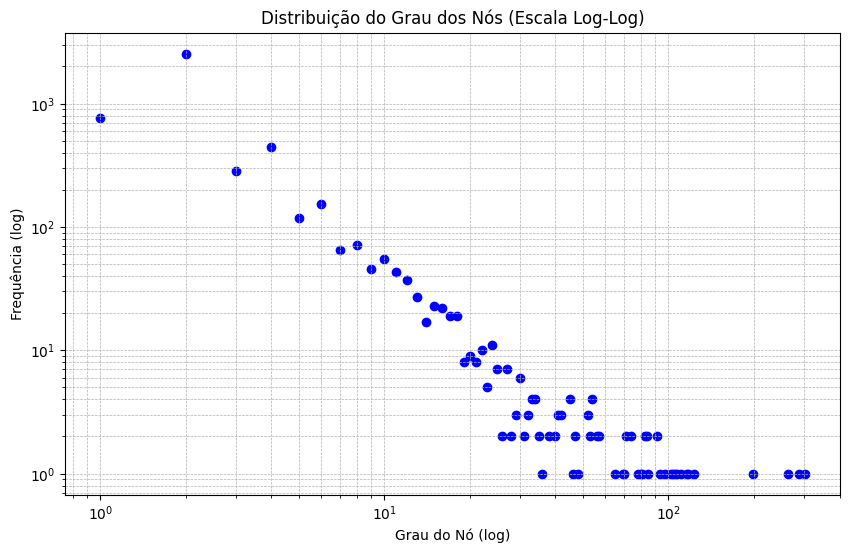
\includegraphics[width=0.8\textwidth]{grauno.png}
    \caption{Distribuição de grau dos nós da rede (em escala log-log).}
    \label{fig:dist_grau}
    Grau médio ($\langle k \rangle$): 4.52.
\end{figure}

\subsection{Componentes do Grafo}
O grafo analisado possui 10 componentes conexos distintos, conforme apresentado na Tabela 1. Destaca-se a presença de um componente gigante, o Componente 1, que contém 4873 nós e 11056 arestas, concentrando a grande maioria dos elementos da rede. Os demais componentes são significativamente menores, com tamanhos variando entre 2 e 7 nós.

A existência de um componente gigante indica que a maior parte dos nós está fortemente conectada, formando uma estrutura coesa que permite o fluxo de informações ou relações entre seus elementos. Já os múltiplos componentes menores representam subgrafos isolados ou pouco conectados, que podem corresponder a grupos específicos ou palavras que não se relacionam diretamente com o núcleo principal da rede, ou seja, pouco usuais.

\begin{table}[H]
\centering
\begin{tabular}{|c|c|c|}
\hline
\textbf{Componente ID} & \textbf{Nº de Nós} & \textbf{Nº de Arestas} \\
\hline
1 & 4873 & 11056 \\
\hline
2 & 7    & 6     \\
\hline
3 & 7    & 6     \\
\hline
4 & 7    & 6     \\
\hline
5 & 4    & 3     \\
\hline
6 & 3    & 2     \\
\hline
7 & 2    & 1     \\
\hline
8 & 2    & 1     \\
\hline
9 & 2    & 1     \\
\hline
10 & 2   & 1     \\
\hline
\end{tabular}
\caption{Distribuição do tamanho dos componentes do grafo.}
\end{table}

\subsection{Coeficiente de Clusterização}
O coeficiente de clusterização global (médio) do grafo é $0{,}0512$. Em uma escala absoluta de $0$ a $1$, esse valor pode parecer baixo, mas sua real significância aparece quando o comparamos com o valor esperado para uma rede aleatória com o mesmo número de nós e grau médio.

No caso de uma rede aleatória (modelo de Erdős-Rényi), o coeficiente de clusterização esperado ($C_{\text{rand}}$) pode ser estimado como:

\[
C_{\text{rand}} \approx \frac{\langle k \rangle}{N}
\]

Com grau médio $\langle k \rangle = 4{,}52$ e aproximadamente $N = 4900$ nós, o valor esperado seria cerca de $0{,}001$. Isso significa que o coeficiente observado é aproximadamente $50$ vezes maior do que o esperado para uma rede aleatória. Tal diferença indica uma estrutura não aleatória, com forte tendência à formação de \textit{clusters} ou "panelinhas".

Além disso, a distribuição dos coeficientes de clusterização locais revela a presença de muitos nós com valor igual a zero, indicando que esses nós são periféricos e possuem poucas conexões entre seus vizinhos. Esses elementos frequentemente atuam como pontes locais, conectando diferentes palavras ou grupos que, de outra forma, permaneceriam isolados. 

\begin{figure}[H]
    \centering
    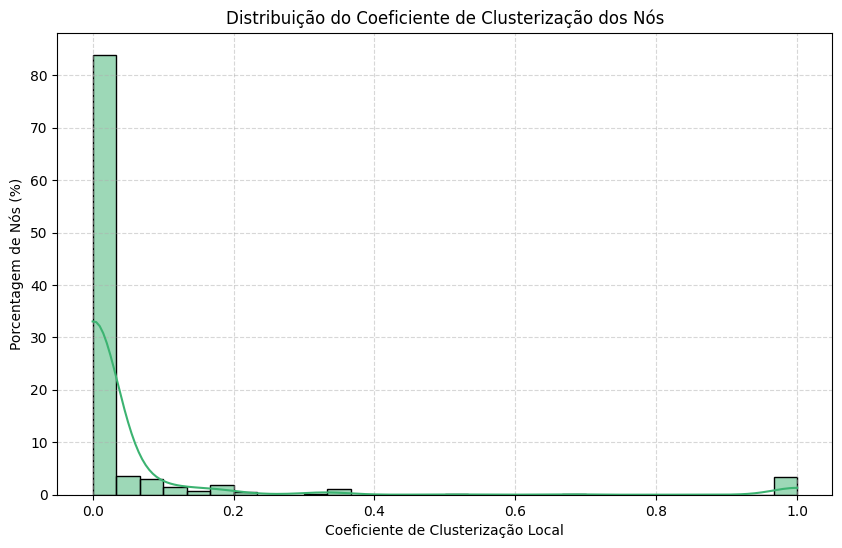
\includegraphics[width=0.8\textwidth]{cluster.png}
    \caption{Distribuição do coeficiente de clusterização dos nós.}
    \label{fig:dist_cluster}
Coeficiente de clusterização global ($C$): 0.0512.
\end{figure}


\subsection{Overlap da Vizinhança}
A predominância de valores iguais a 0,0 no Coeficiente de Jaccard para a maioria dos pares de nós não conectados indica que esses pares compartilham poucos ou nenhum vizinho em comum. Essa característica sugere que a rede apresenta uma estrutura modular ou fragmentada, na qual os nós estão organizados em grupos relativamente isolados, com baixa sobreposição entre as vizinhanças. Em contextos como grafos de coocorrência de palavras, isso revela que a maioria das palavras ocorre em contextos distintos, o que reforça a especificidade e a dispersão da rede. Além disso, essa baixa similaridade local entre nós implica que a probabilidade de formação de novas conexões entre esses pares é pequena, evidenciando uma rede estruturalmente esparsa e altamente segmentada.

\begin{figure}[H]
    \centering
    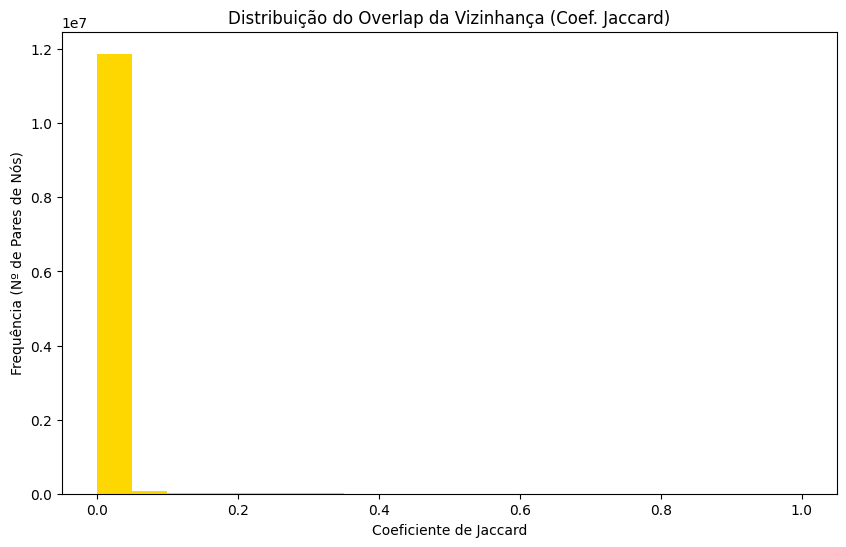
\includegraphics[width=0.6\textwidth]{dist.png}
    \caption{Distribuição do overlap da vizinhança.}
    \label{fig:dist_overlap}
\end{figure}

\subsection{Distâncias na Rede}
A distância média entre os nós no maior componente conectado da rede é 4,35, indicando que, em média, é necessário percorrer pouco mais de quatro arestas para ir de um nó a outro dentro desse componente. Essa medida sugere que a rede possui uma boa conectividade global, permitindo a comunicação eficiente entre os elementos. A distribuição das distâncias apresenta um padrão típico de redes complexas: a maior parte dos pares de nós está separada por pequenas distâncias, enquanto poucas conexões ocorrem em distâncias maiores, decrescendo gradativamente até a distância máxima observada de 18. Essa distribuição confirma que a rede exibe o fenômeno conhecido como "mundo pequeno" (small-world), caracterizado por caminhos curtos entre a maioria dos nós, mesmo em redes de grande escala.

\begin{figure}[H]
    \centering
    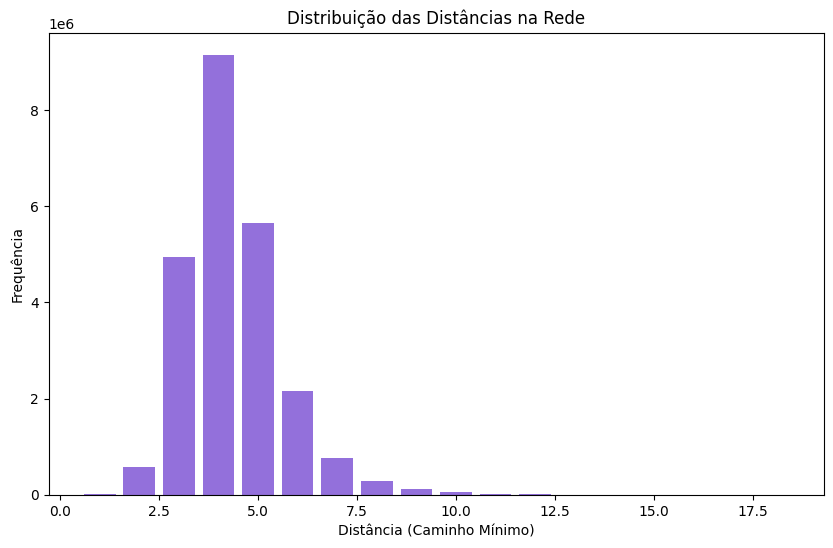
\includegraphics[width=0.8\textwidth]{distancias.png}
    \caption{Distribuição das distâncias entre os nós da rede.}
    \label{fig:dist_distancias}
Distância média no maior componente conectado ($l$): 4.35.
\end{figure}


\subsection{Visualização do Grafo}

 O grafo correspondente ao maior componente conexo é grande demais para permitir uma análise visual eficaz, enquanto os demais componentes são extremamente pequenos e irrelevantes. Por isso, a visualização direta do grafo não é a abordagem mais adequada para compreender sua estrutura.
\begin{figure}[H]
    \centering
    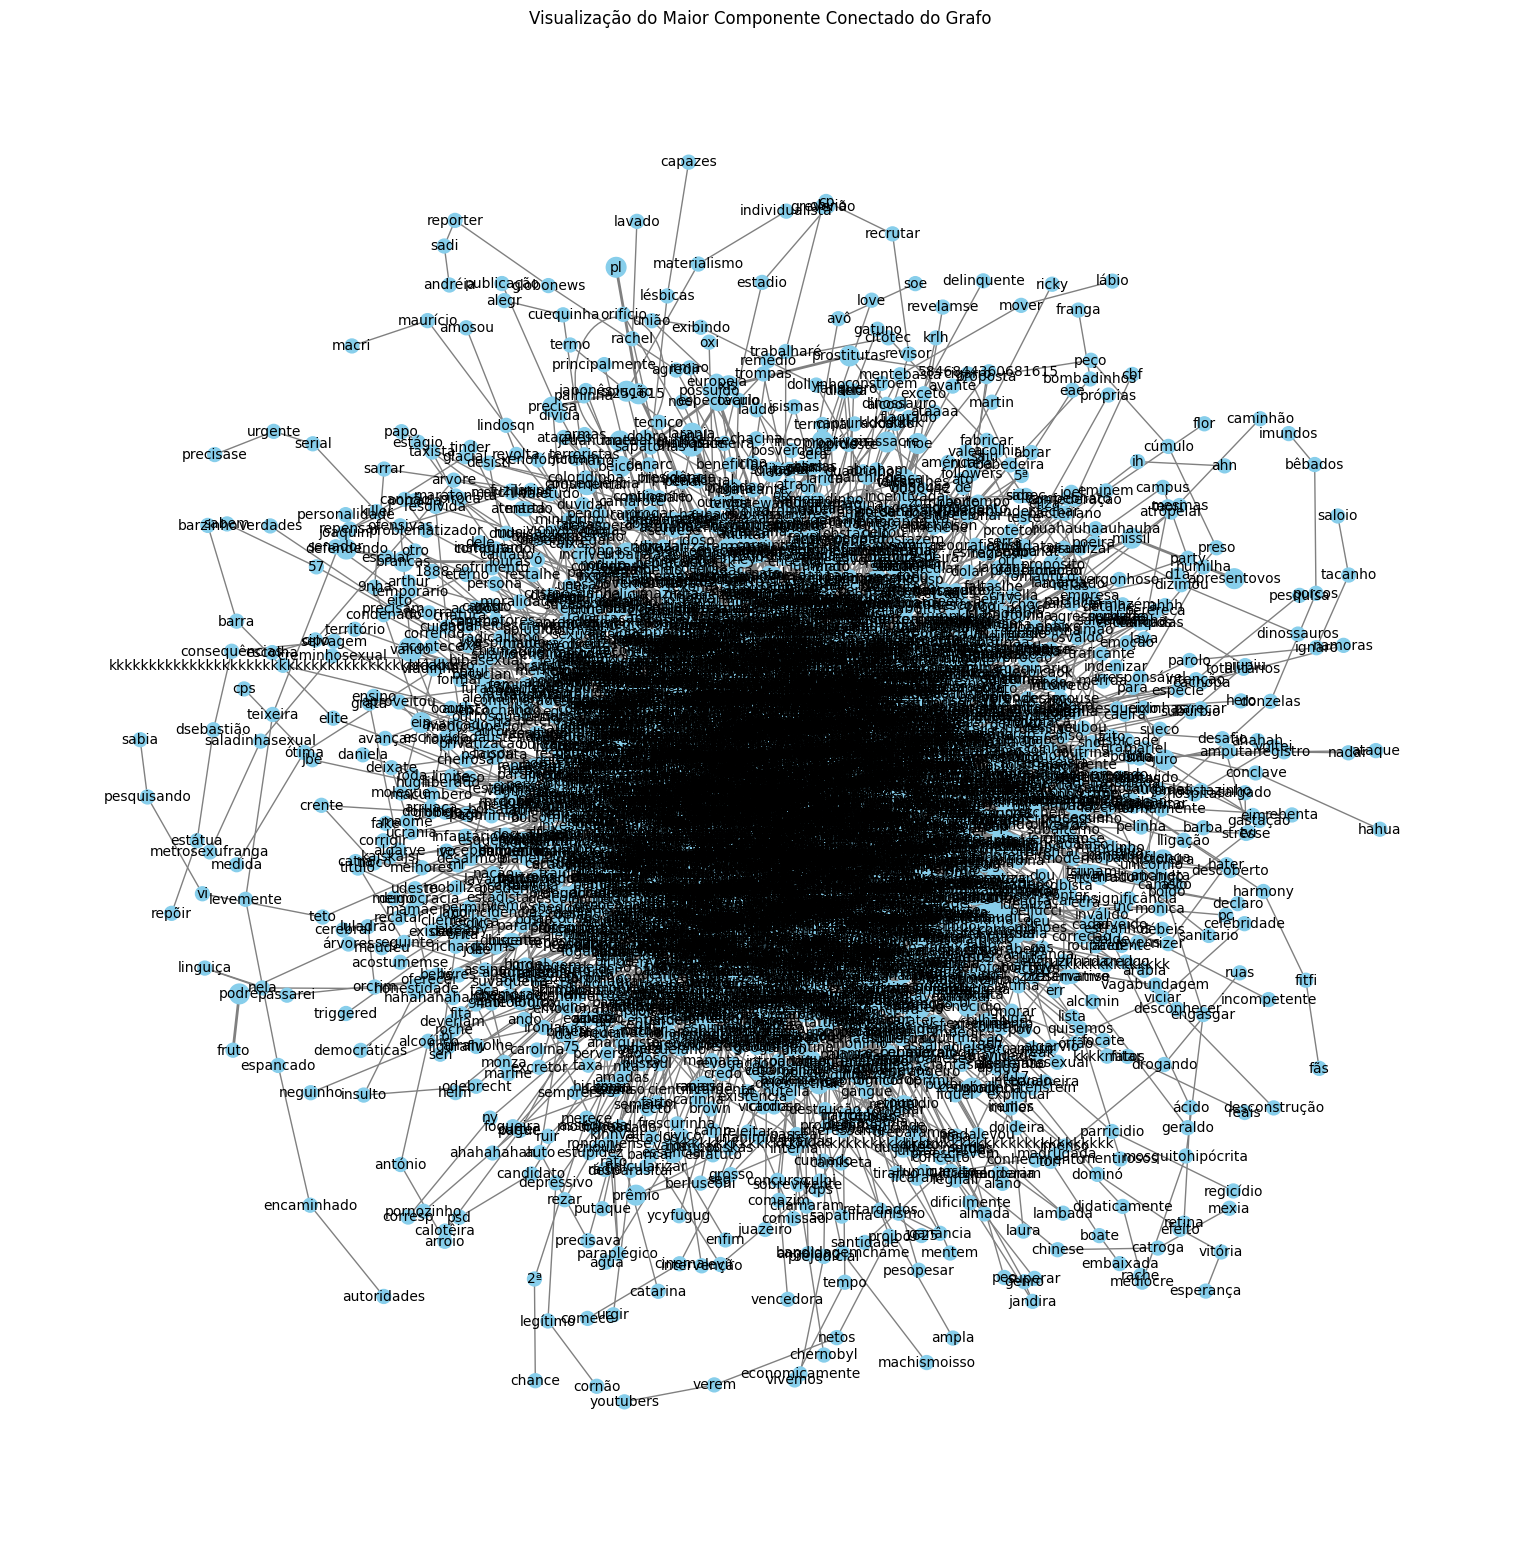
\includegraphics[width=\textwidth]{grafo.png}
    \label{fig:visualizacao}
    \caption{Visualização do componente gigante da rede.}
\end{figure}


\newpage
%%%%%%%%%%%%%%%%%%%%%%%%%%%%%%%%%%%%%%%%%%%%%%%%%%%%%%%%%%%%%%%%%%%%%%%%%%%%%%%%
% Seção 3: Código Fonte
%%%%%%%%%%%%%%%%%%%%%%%%%%%%%%%%%%%%%%%%%%%%%%%%%%%%%%%%%%%%%%%%%%%%%%%%%%%%%%%%
\section{Código Fonte}

Todo o código‑fonte está disponível em um repositório público no GitHub.

\begin{itemize}
    \item \textbf{Repositório (preferencial):} \href{https://github.com/LorenaSouzaMoreiraa/RedesComplexas-TpIntermediario}{\textt{github.com/LorenaSouzaMoreiraa/RedesComplexas-TpIntermediario}}
    \item \textbf{Anexo (alternativo):} Também incluímos um arquivo compactado com o código no envio do trabalho.
\end{itemize}


% Exemplo de como anexar código:
% \begin{lstlisting}[language=Python, caption={Exemplo de código para cálculo de grau médio.}, label={lst:codigo_exemplo}]
% import networkx as nx
%
% # G é o grafo criado nas seções anteriores
% average_degree = sum(dict(G.degree()).values()) / G.number_of_nodes()
% print(f"O grau médio do grafo é: {average_degree}")
% \end{lstlisting}

%%%%%%%%%%%%%%%%%%%%%%%%%%%%%%%%%%%%%%%%%%%%%%%%%%%%%%%%%%%%%%%%%%%%%%%%%%%%%%%%
% --- PARTE FINAL DO DOCUMENTO ---
%%%%%%%%%%%%%%%%%%%%%%%%%%%%%%%%%%%%%%%%%%%%%%%%%%%%%%%%%%%%%%%%%%%%%%%%%%%%%%%%

% O comando \backmatter indica que a parte principal do trabalho terminou
% e que agora virão os apêndices, referências, etc.
\backmatter 
\newpage
% --- SEÇÃO DE REFERÊNCIAS ---
\bibliography{referencias} % Indica o nome do seu arquivo .bib (sem a extensão)

\end{document}